\documentclass [a4 paper, 11pt, titlepage] {article}

\usepackage{nicematrix}
\usepackage{graphicx}
\usepackage{IEEEtrantools}
\usepackage{multirow}
\usepackage{caption}
\usepackage{subcaption}

\addtolength{\hoffset}{-2cm}
\addtolength{\textwidth}{4cm}

\begin{document}
	\title{EE568 Project 4}
	\author{Baris Kuseyri}
	\date{\today}
	\maketitle
	
	\pagenumbering{arabic}
	\tableofcontents
	\newpage
	
	\section{Introduction}

	FSCW IPMSM type EM are reported to exhibit very high torque densities, impressive fault-tolerant capabilities and low cogging torque when deployed correctly. In the last decade, they have become the most popular topologies in electric vehicles due to these characteristics. Extensive research have been performed on this topic, and with their remarkable efficiency ratings, they are currently the prime candidate for a greener world with electric transportation.

	\subsection{Aims \& Objectives}
	This paper designs an electric motor (EM) to be used as a part of an hybrid electric propulsion system for Cessna 172 Skyhawk. Definition of the hybrid electric propulsion system and the corresponding EM requirements, e.g. rated power, dimensional limitations etc., are outlined in the project proposal. Several EMs with different slot/pole combinations are designed, complying the described requirements. A comparative analysis is performed on these designs, focusing on cogging torque aspect. One design is chosen, and further alterations are applied to enhance the EM performance.


	\section{Literature Review}
	The term FSCW is used to indicate that EM has a non-integral number of slots-per-pole-per-phase $q$,
	\begin{IEEEeqnarray*}{rCl}
		q = \frac{Q}{2pm}
	\end{IEEEeqnarray*}
	where, $Q$ is number of slots, $2p$ is number of poles and $m$ is number of phase.
	
	FSCW topologies are reported to exhibit higher power density. CW comprises of shorter end-windings, resulting with a lower copper loss due to end-windings, compared to DW. FSCW topologies display higher self-inductance, leading to a wider field-weakening region \cite{farshadnia_advanced_2018}.
	The aspect of fault-tolerant in an EM is proportional to several characteristics.	First, magnetic coupling between phases, which implies a high mutual inductance, diminishes the fault-tolerancy of an EM. Therefore, phases which are magnetically seperated is desired to achieve a higher fault-tolerancy rating \cite{bianchi_use_2006}. In SPM machines, single-layer winding demonstrates higher self-inductances and lower mutual inductances compared to its double-layer counterparts. A high self-inductance limits the amplitude of short-circuit current, a significant property for fault-tolerancy \cite{el-refaie_fractional-slot_2010} \cite{ishak_comparison_2006}. Additionally, it is desired to have phases which are physically seperated to achieve fault-tolerancy \cite{bianchi_use_2006}. In CW topologies, there exists one unwounded stator tooth between two coils, physically seperating each phase.
	\subsection{Cogging Torque}
	3 torque components are present in FSCW PMSM. These are: alignment torque, reluctance torque and cogging torque.
	\begin{IEEEeqnarray*}{rCl}
		T_{em}(t)=T_{align}(t)+T_{rel}(t)+T_{cog}(t)
	\end{IEEEeqnarray*}
	Cogging torque is one of the torque elements contributing to the torque ripple in the PMSM. The amount of stator teeth aligned with poles in the rotor at a given instance. For the corresponding magnetic circuit, permeance is highest when a rotor pole and a stator tooth are aligned. The system is stable at this point, and the corresponding cogging torque is zero. This results with a force that tries to keep the pole steady; hence, emerging a torque counter to the rotor rotation. This is called 'cogging torque'. More of such alignments result with more cogging torque. 
	The most acknowledged indicator for the cogging torque in a PMSM is the value of least common multiple (LCM) between the number of slots $Q$ and number of poles $2p$. Zhu and Howe (2000) introduce a factor $C_T=\frac{2pQ}{LCM(Q,2p)}$, to assess the cogging torque in a given PMSM. They profess that this factor $C_T$ is directly proportional to the amplitude of the cogging torque \cite{zhu_influence_2000}. Zhu (2011) claims the same as Zhu and Howe (2000), stating that higher LCM and lower GCM between number of slots $Q$ and number of poles $2p$ lead to lower cogging torque. In addition to this, it is argued that machines with a slot/pole combination of $2p=Q\pm2$ exhibit very low cogging torque, while machines with a slot/pole combination of $2p=Q\pm1$ exhibit the lowest cogging torque, with a downside of having unbalanced magnetic force \cite{masmoudi_fractional_2011}. Zhu, Wu and Jamil (2014) inspect machines with slot/pole combinations of $2p=Q\pm2$, $2p=Q\pm1$, $Q/2p=12/8$ and one integer-slot machine $Q/2p=12/4$, assessing the machines in terms of cogging torque, leading to a similar result \cite{zhu_influence_2014}. Jahns and Soong (1996) examine cogging torque in different machines and provide various methods to reduce the cogging torque \cite{jahns_pulsating_1996}. They state that skewing is one of the most popular and most effective way to reduce the cogging torque, if not, eliminate completely. Azar, Zhu and Ombach (2012) utilize skewing method in their work, to reduce the cogging torque. They report that skewing the PMSM by one actual cogging torque period can eliminate the cogging torque and reduce the torque ripple significantly \cite{azar_influence_2012}. Jahns and Soong also mention about winding distribution, increasing number of phases and air-gap winding and their effect on reducing cogging torque when carefully employed \cite{jahns_pulsating_1996}. Additionally, they report the effect of magnet arc width and positioning and its effect on cogging torque \cite{jahns_pulsating_1996}. Work of Ahsanullah, Dutta and Rahman (2013) and Wang, Wang and Jung (2013) show how magnet arc width may reduce the resulting cogging torque \cite{wang_cogging_2013} \cite{ahsanullah_design_2013}. Jahns and Soong (1996) also report the utilization of dummy slots and dummy teeth and how it may result with the reduction of cogging torque \cite{jahns_pulsating_1996}. Zhu and Howe (2000) work on this method, naming not as dummy, but auxiliary, and approve this method for reducing the cogging torque. Bianchi and Bolognani (2002) reports a similar work to Jahns and Soong (1996), reporting similar methods and similar results, with an additional method of PM shifting. Wu and Zhu (2015) reports the effect of tooth tip width on cogging torque and torque ripple in FSCW SPM, and the trade-off between the two torque components in such machine \cite{wu_design_2015}. Finally, Farshadnia (2018) reports similar cogging torque characteristics as Zhu and Howe (2000), reporting in his work about how higher LCM between number of slots $Q$ and number of poles $2p$ indicates lower cogging torque.
	
	\section{Analytical Calculation \& Sizing}
	As mentioned in the proposal the machine ratings are,
	\begin{table}[h]
		\begin{center}
			\begin{tabular}{c|c|c}
				Power [kW] &  Speed [rad/s] &  Torque [N$\cdot$m]\\
				\hline
				$46.9790$ & $282.7433$ & $166.1542$
			\end{tabular}
		\end{center}
		\caption{Required EM Ratings}
		\label{fig:EMratings}
	\end{table}
	

	
	\subsection{Magnetic Loading \& Electrical Loading}
	According to Pyrhonen et al., permitted RMS values for linear current densities $\bar{A}$, current densities $J$ and peak air-gap flux densities $\hat{B}_g$ for PMSMs with single-layer field winding, and the corresponding tangential stress $\sigma_{Ftan}$ are reported as given in Tab. \ref{fig:EMoperations}.
	\begin{table}[h]
		\begin{center}
			\begin{tabular}{c|c|c|c||c}
				 & $\bar{A}$ $[kA/m]$ & $\hat{B}_g$ $[T]$ & $J$ $[A/mm^2]$ & $\sigma_{Ftan}$ $[Pa]$ \\
				\hline
				Provided Range & 35-65 &  0.85-1.05 & 2-4 & 21000-48000\\
				Chosen Values & 50 &  0.95 &  & 33876\\
			\end{tabular}
		\end{center}
		\caption{PMSMs with Single-Layer Field Winding \cite{pyrhonen_design_2014}}
		\label{fig:EMoperations}
	\end{table}
	
	Here, $\sigma_{Ftan}$ is calculated by
	\begin{equation}
		\sigma_{Ftan}=\frac{\hat{A}\hat{B}_g}{2}=\frac{\bar{A}\hat{B}_g}{\sqrt{2}}
	\end{equation}
	
	where, ($\hat{\cdot}$) is for peak value and ($\bar{\cdot}$) is for RMS value of the parameter.
	Therefore, suitable magnetic and electric loading are chosen as the midpoint of the ranges provided. The chosen values can be seen in Tab. \ref{fig:EMoperations}.
	
	\subsection{Specific Machine Constant}
	Specific machine constant is a factor that can be used to assess the EM performance \cite{pyrhonen_design_2014}. It includes the tangential stress on the rotor, as well as the winding factor. The equation for specific machine constant is given in Eq. 
	
	\begin{equation}
		C=\frac{\pi^2}{\sqrt{2}}k_w\bar{A}\hat{B}_g=\frac{\pi^2}{2}k_w\hat{A}\hat{B}_g
	\end{equation}
	where, $k_w$ is the winding factor.
	
	
	\subsection{Rough Dimensions}
	
	
	\paragraph{Rotor Volume $V_r$} can be calculated from the torque equation shown in Eq. \ref{eq:torqueEquation}.
	\begin{equation}
		T=\sigma_{Ftan}r_r(2\pi r_rl')=\sigma_{Ftan}V_r 
		\label{eq:torqueEquation}	
	\end{equation}
	\begin{equation}
		V_r=\pi\frac{D^2_r}{2}l'=\frac{T}{2\sigma_{Ftan}}
	\end{equation}
	where, $l'$ is the effective axial length, which is defined as $l'=l+2l_g$, where $l$ is the actual axial length.

	\paragraph{Air-gap Clearance} in PMSMs can be calculated in a similar manner with asynchronous machines
	\begin{equation}
		\delta_g=\frac{0.18+0.006P^{0.4}}{1000} [m]
	\end{equation}
	where, $P$ represents the rated power of the EM. As the power rating of each EM designed are same, each of the machine has the same air-gap clearance.
	
	\paragraph{Equivalent Machine Length to Air-gap Diameter $\chi=\frac{l'}{D_g}$} in synchronous machines with pole-pair number more than 1, i.e. $p>1$, this ratio is calculated as
	\begin{IEEEeqnarray*}{rCl}
		\chi &=& \frac{l'}{D_g}\approx\frac{\pi}{4p}\sqrt{p} \\
	\end{IEEEeqnarray*}
	where, the $p$ stands for number of pole pairs in the machine. $\chi$ ratio for different number of pole-pairs $p$ can be seen in Fig. \ref{fig:chiRatio}.
	\begin{figure}[h]
		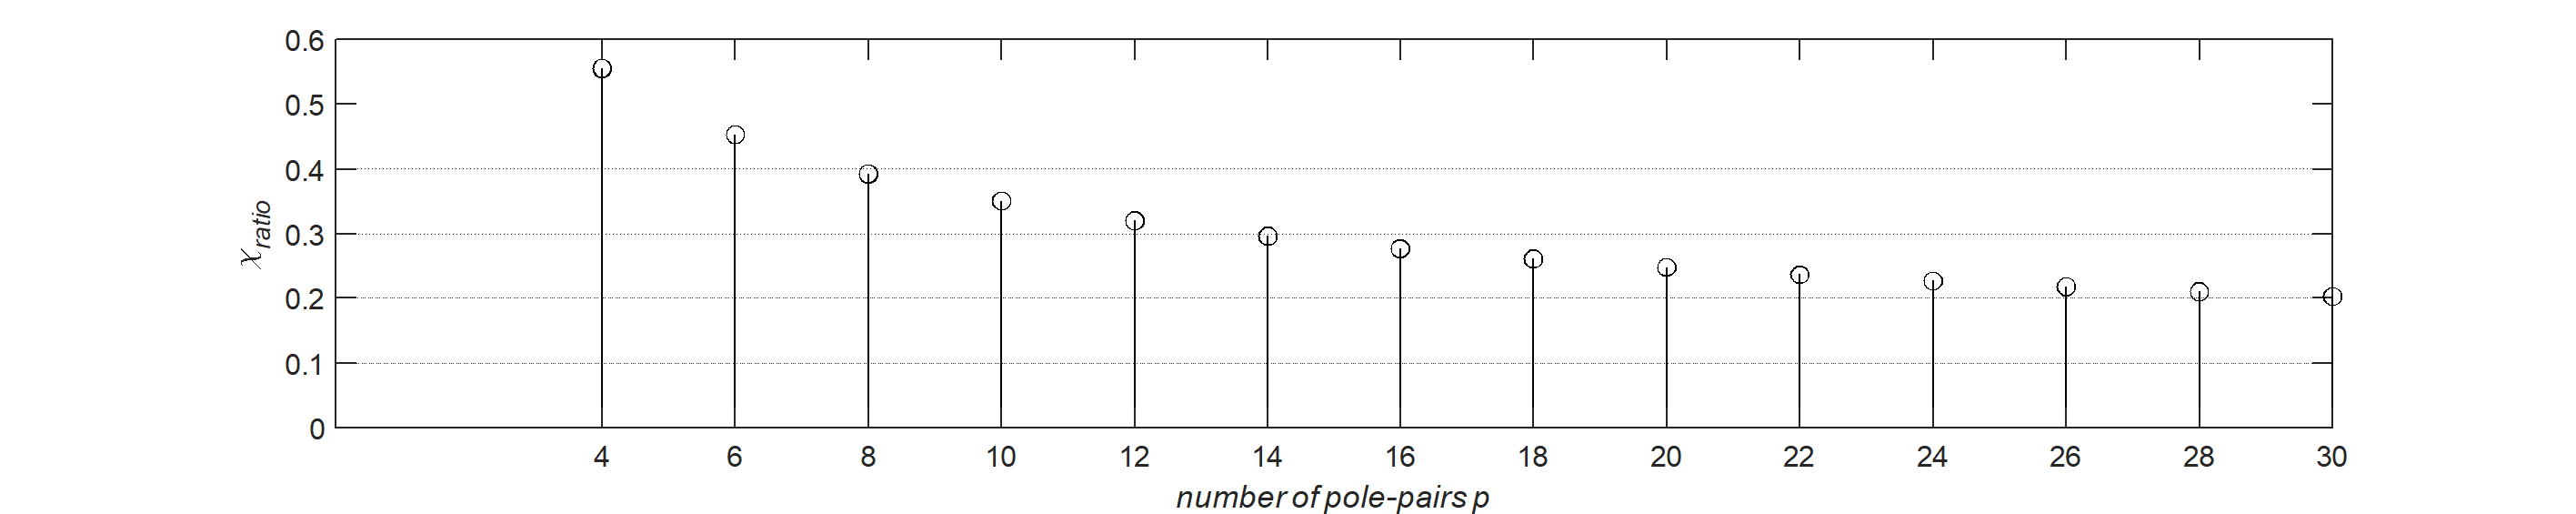
\includegraphics[width=\textwidth]{chiRatio.png}
		\caption{$\chi$ ratio for different number of pole-pairs $p$}
		\label{fig:chiRatio}
	\end{figure}
	
	
	\subsection{Winding Configurations}
	This paper analyses single-layer FSCW winding configurations. In this manner, topologies with number of slots as $Q=18, 24$, and number of poles as $2p=16, 20, 22, 26, 28$ are inspected. These slot/pole combinations and their corresponding winding factors are presented in Table \ref{tab:windingConf}.
	\begin{table}[h]
		\begin{center}
			$\begin{NiceArray}{|C|C|C|C|C|}[first-row,first-col]
				Q/2p & 16 & 20 & 22 & 26 & 28 \\
				\hline
				18 & 0.945 & 0.945 & 0.902 & 0.735 & 0.617 \\
				\hline
				24 & 0.866 & 0.966 & 0.958 & 0.958 & 0.966 \\
				\hline
			\end{NiceArray}$
		\end{center}
		\caption{Winding Configurations and corresponding Winding Factors $k_w$}
		\label{tab:windingConf}
	\end{table}	
	
	\subsection{Machine Parameters}
		
	\paragraph{Split Ratio $\lambda$} is the ratio of rotor outer diameter to stator outer diameter $s=D_{ro}/D_{so}$. Wu et al. derives the optimal split ratio for IPM machines with non-overlapping windings using torque density equation \cite{wu_optimal_2010}. First, a flux density ratio $\gamma$ is defined as the ratio of air-gap flux density to maximum flux density the stator lamination can support before magnetically saturating. Split ratio $\lambda$, flux density ratio $\gamma$ and another intermediary ratio $k$ is defined in \ref{eq:Wulambdagammak}. The expression derived for the optimal split ratio is
	
	\begin{IEEEeqnarray*}{rCl}
		B_g=\frac{3\sqrt{3}}{2\pi}B_{gmax}
	\end{IEEEeqnarray*}
	\begin{align}
		\gamma&=\frac{B_g}{B_{max}} & k&=\frac{p}{Q}
		\label{eq:Wulambdagammak}
	\end{align}
	where, $D_{ro}$ is rotor outer diameter, $D_{so}$ is stator outer diameter, $B_g$ is the average airgap flux density, $p$ is the number of pole-pairs and $Q$ is the number of slots. Then, the optimal split ratio expression is derived as
	\begin{IEEEeqnarray*}{rCl}
		\lambda=\frac{D_{ro}}{D_{so}}=\frac{-b_1-\sqrt{b^2_1-4a_1}}{2a_1}
	\end{IEEEeqnarray*}
	\begin{align*}
		a_1&=2\big[\frac{k\pi}{p}(\frac{k\pi}{p}+2)\gamma^2+2\gamma-1\big] & b_1&=-3(\frac{k\pi}{p}+1)\gamma
	\end{align*}
	
	\paragraph{Teeth/slot opening} this paper utilizes parallel teeth topology with a slot opening to tooth width ratio of 50:50. This means that at the inner side of the stator, the section on the stator retained for one slot and one tooth is divided equally between those two. Therefore, the tooth width is
	\begin{equation}
		\tau_{tooth,i}=\tau_{tooth,o}=\frac{\pi D_{si}}{2Q}=\tau_{tooth}=\tau_{slot,inner}
	\end{equation}
	where, $D_{si}$ is the stator inner diameter.
	
	\paragraph{Back-core thickness} are set to be equal to the tooth width of the EMs. In single-layer FSCW topologies, phases are magnetically decoupled, meaning that the flux runs through coupled adjacent poles. Therefore, the flux travels through one tooth continues its path through the back iron to the adjacent tooth and the corresponding pole, without interacting with other flux paths at the back iron. Therefore, back-iron thickness doesn't have to be higher than the tooth thickness. 
	\begin{equation}
		h_{back-iron}=\tau_{tooth}
	\end{equation}

	\paragraph{Teeth/slot height} can be calculated by
	\begin{equation}
		h_{tooth}=h_{slot}=\frac{D_{so}}{2}-h_{back-iron}-\frac{D_{ro}}{2}-\delta_g
	\end{equation}
	
	\paragraph{Slot outer length} can be calculated by
	\begin{equation}
		\tau_{slot,outer}=\frac{\pi (D_{so}-2h_{back-iron})}{Q}-\tau_{tooth}
	\end{equation}
	
		\begin{table}[h]
		\begin{center}
			\begin{tabular}{c|c}
				 &  \\
				\hline
				back-core thickness & 19.07mm \\
				number of coils & \\
				cable size & 
			\end{tabular}
		\end{center}
		\caption{Machine Parameters}
		\label{tab:machineParameters}
	\end{table}
	
	\paragraph{Slot tip width} is determined to be $4mm$ more than the tooth width for each of the designs.
	
	\paragraph{Rotor IPM parameters}
	The rotor side is designed to be equivalent in each of the designs. In each pole, magnet width is determined such that the magnet arc is 0.6 of the pole arc. The pole embrace is also determined to be 0.6, equal to the magnet arc. The bridge is $1mm$ and the rib is $2mm$. Magnet length is determined in each EM to achieve an air-gap flux density $B_g=0.95T$. The magnet widths can be seen in Tab. \ref{tab:EMparameters} and magnet lengths can be seen in Tab. \ref{tab:resultslvl1}.
	
	\subsection{Material selection}
	
	\paragraph{Magnet Material} There are no cost limitations to the EM application. The required air-gap flux density $B_g=0.95T$, a high value for a flat-shaped IPM topology. According to Eclipse Magnetics, N35 grade PMs have the VH/AH choice, in which the magnet can operate up until the temperatures of $230^{\circ}C$. This is not a requirement for the application, however, implementing N35 PM magnets omits the machine's operable temperature range dependency to the PM magnet demagnetization due to heat. Therefore, N35 grade NdFeB magnets are tried first. However, the required air-gap flux density is not achieved with these PMs. Thus, PMs with higher remanence flux density $B_r$ are chosen. N50 grade PMs by Arnold Magnetics are chosen for the application. N50 grade NdFeB magnet characteristics are given in Table. \ref{tab:N50}
	
	\begin{table}[h]
		\begin{center}
			\begin{tabular}{c|c|c}
				$B_r$ [$mT$] & $H_c$ [$kA/m$] & Max. Energy BHMax [$kJ/m^3$] \\
				\hline
				1.3471 & -962.042 & 346.972
			\end{tabular}
		\end{center}
		\caption{N50 grade NdFeB PM characteristics}
		\label{tab:N50}
	\end{table}
	where, $B_r$ is remanence flux density and $H_c$ is coercivity.
	
	\paragraph{Lamination Material} There are no cost limitations to the EM application. AK Steel M15 14mil steel is chosen for both stator and rotor side of the designs. The steel saturates at around $2T$. 
	
	
	
	
	
	
	\subsection{Electrical circuit parameter}
	
	\paragraph{Flux per Pole}
	Flux per pole can be calculated by


	
	
	\subsection{Overall}
	
	The chosen EM parameters are given in Tab. \ref{tab:EMparameters}. As described above, the linear current density $J$ is calculated by utilizing the method provided by Wu et al. to calculate optimal split ratio $D_r/D_s$, which can be seen in Tab. \ref{tab:resultingStatorSlotRatios} for each of the slot/pole configurations \cite{wu_optimal_2010}. The resulting linear current density $J$ values calculated, for each of the slot/pole combinations analysed, are satisfying the linear current density $J$ range suggested by Pyrhonen et al., that is $2 [A/mm^2]<J [A/mm^2]<4 [A/mm^2]$ for single-layer PMSMs with field windings \cite{pyrhonen_design_2014}. Furthermore, the split ratio calculated via. the method proposed by Wu et al. denies what Soong comments on stator slot ratio, that is the ratio of stator inner diameter to slot outer diameter \cite{pellegrino_rediscovery_2016-1}. Soong shows how in parallel tooth stator topologies, the resulting electromagnetic torque $T_{em}$ peaks when stator slot ratio is $d=1/\sqrt{3}\approx0.58$. Additionally, Soong comments how the stator slot ratio may increase up to 0.8 in EMs with high number of poles. Each of the stator slot ratio calculated via the method provided by Wu et al. are above 0.8. The slot/pole combinations with least amount of poles have a pole number of 16, which is high. The peculiar result, however, is that the stator slot ratio decreases as pole number increases, according to the results calculated via the method provided by Wu et al. \cite{wu_optimal_2010}.
	
	\begin{table}[h]
		\begin{center}
			\begin{tabular}{c|c|c|c|c|c}
				$Q=18$ & $p=16$ & $p=20$ & $p=22$ & $p=26$ & $p=28$ \\
				\hline
				Stator Slot Ratio $d$ & 0.8338 & 0.8337 & 0.8337 & 0.8336 & 0.8336 \\
				\hline\hline
				$Q=24$ & $p=16$ & $p=20$ & $p=22$ & $p=26$ & $p=28$ \\
				\hline
				Stator Slot Ratio $d$ & 0.8283 & 0.8282 & 0.8282 & 0.8281 & 0.8281 \\
			\end{tabular}
		\end{center}
		\caption{Stator Slot Ratios Calculated via method provided by Wu et al. \cite{wu_optimal_2010}}
		\label{tab:resultingStatorSlotRatios}
	\end{table}
	
	
	
	\begin{table}[h]
		\begin{center}
			\begin{tabular}{c|c|c|c|c|c}
				Magnetic Loading $\hat{B}[T]$ & \multicolumn{5}{c}{0.95} \\
				Electric Loading $\hat{A}[A/m]$ & \multicolumn{5}{c}{50000} \\
				Tangential Stress $\sigma_{Ftan}[Pa]$ & \multicolumn{5}{c}{33876} \\
				Rotor Volume $V_r [m^2]$ & \multicolumn{5}{c}{0.002473447965892} \\
				Air-gap Clearance $\delta_g [mm]$ & \multicolumn{5}{c}{0.624} \\
				\hline\hline
				$Q=18$ & $p=16$ & $p=20$ & $p=22$ & $p=26$ & $p=28$ \\
				\hline
				Linear Current Density $J [A/mm^2]$ & 3.27 & 3.15 & 3.10 & 3.02 & 2.98 \\
				Specific Machine Constant $[kWs/m^3]$ & 313264 & 313264 & 299009 & 243650 & 204533 \\
				Axial Length $l [mm]$ & 49.6 & 46.1 & 44.6 & 42.2 & 41.2 \\
				Winding Factor $k_w$ & 0.945 & 0.945 & 0.902 & 0.735 & 0.6170 \\
				Rotor outer diameter $D_{ro} [mm]$ & 252.2 & 261.7 & 265.9 & 273.4 & 276.8 \\
				Stator inner diameter $D_{si} [mm]$ & 253.4 & 263.0 & 267.2 & 274.7 & 278.1 \\
				Stator outer diameter $D_{so} [mm]$ & 398.5 & 413.6 & 420.2 & 432.1 & 437.4 \\
				Tooth width $\tau_{teeth} [mm]$ & \multirow{3}{4em}{22.0} & \multirow{3}{4em}{22.8} & \multirow{3}{4em}{23.2} & \multirow{3}{4em}{23.9} & \multirow{3}{4em}{24.2} \\
				Slot inner width $\tau_{slot,inner} [mm]$ & & & & & \\
				back-iron thickness $h_{back-iron} [mm]$ & & & & & \\
				Tooth height $h_{teeth} [mm]$ & \multirow{2}{4em}{50.5} & \multirow{2}{4em}{52.5} & \multirow{2}{4em}{53.3} & \multirow{2}{4em}{54.8} & \multirow{2}{4em}{55.5} \\
				Slot heigth $h_{teeth} [mm]$ &  &  &  &  & \\
				Slot outer width $\tau_{slot,outer} [mm]$ & 39.9 & 41.4 & 42.0 & 43.2 & 43.8 \\
				Magnet width [mm] & 28.7 & 23.9 & 	22.1 & 19.2 & 18.1 \\
				\hline\hline
				$Q=24$ & $p=16$ & $p=20$ & $p=22$ & $p=26$ & $p=28$ \\
				\hline
				Linear Current Density $J [A/mm^2]$ & 3.96 & 3.81 & 3.75 & 3.65 & 2.60 \\
				Specific Machine Constant $[kWs/m^3]$ & 287076 & 320225 & 317573 & 317573 & 320225 \\
				Axial Length $l [mm]$ & 49.6 & 46.1 & 44.6 & 42.2 & 41.2 \\
				Winding Factor $k_w$ & 0.866 & 0.966 & 0.958 & 0.958 & 0.966 \\
				Rotor outer diameter $D_{ro} [mm]$ & 252.2 & 261.7 & 265.9 & 273.4 & 276.8 \\
				Stator inner diameter $D_{si} [mm]$ & 253.4 & 263.0 & 267.2 & 274.7 & 278.1 \\
				Stator outer diameter $D_{so} [mm]$ & 391.5 & 406.3 & 412.8 & 424.5 & 429.8 \\
				Tooth width $\tau_{teeth} [mm]$ & \multirow{3}{4em}{16.5} & \multirow{3}{4em}{17.1} & \multirow{3}{4em}{17.4} & \multirow{3}{4em}{17.9} & \multirow{3}{4em}{18.1} \\
				Slot inner width $\tau_{slot,inner} [mm]$ & & & & & \\
				back-iron thickness $h_{back-iron} [mm]$ & & & & & \\
				Tooth height $h_{teeth} [mm]$ & \multirow{2}{4em}{52.5} & \multirow{2}{4em}{54.5} & \multirow{2}{4em}{55.4} & \multirow{2}{4em}{57.0} & \multirow{2}{4em}{57.7} \\
				Slot heigth $h_{teeth} [mm]$ &  &  &  &  & \\
				Slot outer width $\tau_{slot,outer} [mm]$ & 29.9 & 31.0 & 31.5 & 32.4 & 32.8 \\
				Magnet width [mm] & 28.7 & 23.9 & 	22.1 & 19.2 & 18.1 \\
			\end{tabular}
		\end{center}
		\caption{Machine Parameters}
		\label{tab:EMparameters}
	\end{table}
	
	
	
	
	\section{FEA Modelling: Comparing Winding Configurations}
		
	\begin{table}[h]
		\begin{center}
			\begin{tabular}{c|c|c|c|c|c}
				$Q=18$ & $p=16$ & $p=20$ & $p=22$ & $p=26$ & $p=28$ \\
				\hline
				Peak air-gap flux density $B_g [T]$ & 0.95436 & 0.94957 & 0.95353 & 0.94894 & 0.94773 \\
				Cogging Torque $T_{cogging} [Nm]$ & 2.53194 & 0.55637 & 2.42117 & 0.90783 & 0.85279\\
				Magnet Length $l_m [mm]$ & 9 & 11 & 13 & 16 & 20 \\
				Cogging Torque Factor $C_T=\frac{2pQ}{LCM(Q,2p)}$ & 2 & 2 & 2 & 2 & 2 \\
				\hline\hline
				$Q=24$ & $p=16$ & $p=20$ & $p=22$ & $p=26$ & $p=28$ \\
				\hline
				Peak air-gap flux density $B_g [T]$ & 0.95240 & 0.95191 & 0.95023 & 0.94801 & 0.94818 \\
				Cogging Torque $T_{cogging} [Nm]$ & 17.4812 & 3.7297 & 0.68872 & 0.10482 & 4.77034 \\
				Magnet Length $l_m [mm]$ & 15 & 12 & 12 & 15 & 18 \\
				Cogging Torque Factor $C_T=\frac{2pQ}{LCM(Q,2p)}$ & 8 & 4 & 2 & 2 & 4 \\
			\end{tabular}
		\end{center}
		\caption{Results: Cogging Torque $T_{cogging}$ for different slot $Q$ and pole $2p$ values}
		\label{tab:resultslvl1}
	\end{table}
	
	The results cogging torque values are given in Tab. \ref{resultslvl1} and can also be seen in Fig. \ref{fig:coggingTorquelvl1}. As can be seen, the cogging torque for PMSMs with slot number $Q=24$ is highest at the PMSM with pole number $2p=16$, which has a cogging torque factor of $C_T=8$. PMSMs with slot/pole combination $Q/2p=24/20$ and $Q/2p=24/28$ exhibit lower cogging torque than former, as their cogging torque factor is $C_T=4$, and PMSMs with slot/pole combination $Q/2p=24/22$ and $Q/2p=24/26$ exhibit lowest cogging torque than former, as their cogging torque factor is $C_T=2$. Amongst all the configurations, each one with a cogging torque factor of $C_T=2$ exhibit lower cogging torque than the ones with cogging torque factor of $C_T>2$. Therefore, the results are consistent with the cogging torque factor $C_T$ analysis introduced by Zhu and Howe (2000) \cite{zhu_influence_2000}.
	
	Each of the PMSMs exhibit a peak air-gap flux density of $B_g=0.95T$. This is important for a fair comparison of cogging torque between each configuration, while cogging torque involves the interaction of the PMSMs with stator tooths, forming up a magnetic circuit with the resulting torque as a function of the circuit's permeance. To achieve such high air-gap flux density with flat-shaped IPMs, magnet width is increased significantly, especially in the configurations with higher pole numbers. The air-gap flux density follows the relation,
	\begin{equation}
		B_g=\frac{B_r}{1+u_r\frac{l_g}{l_m}}
	\end{equation}
	where, $B_g$ is the air-gap flux density, $B_r$ is the remanence flux density value of the magnet, $u_r$ is the magnet relative permeability, $l_g$ is the air-gap clearance and $l_m$ is the magnet width. Therefore, increasing the magnet width does not have a dominant effect on air-gap flux density $B_g$, if $l_m>>l_g$. Therefore, further rotor optimization is necessary. Here, v-shaped PM topology is recommended to achieve such high air-gap flux density $B_g$ values, as the flux concentration effect of the topology may provide the aimed air-gap flux density $B_g$ values with acceptable amount of PM material.
	
	
	\begin{figure}[h]
		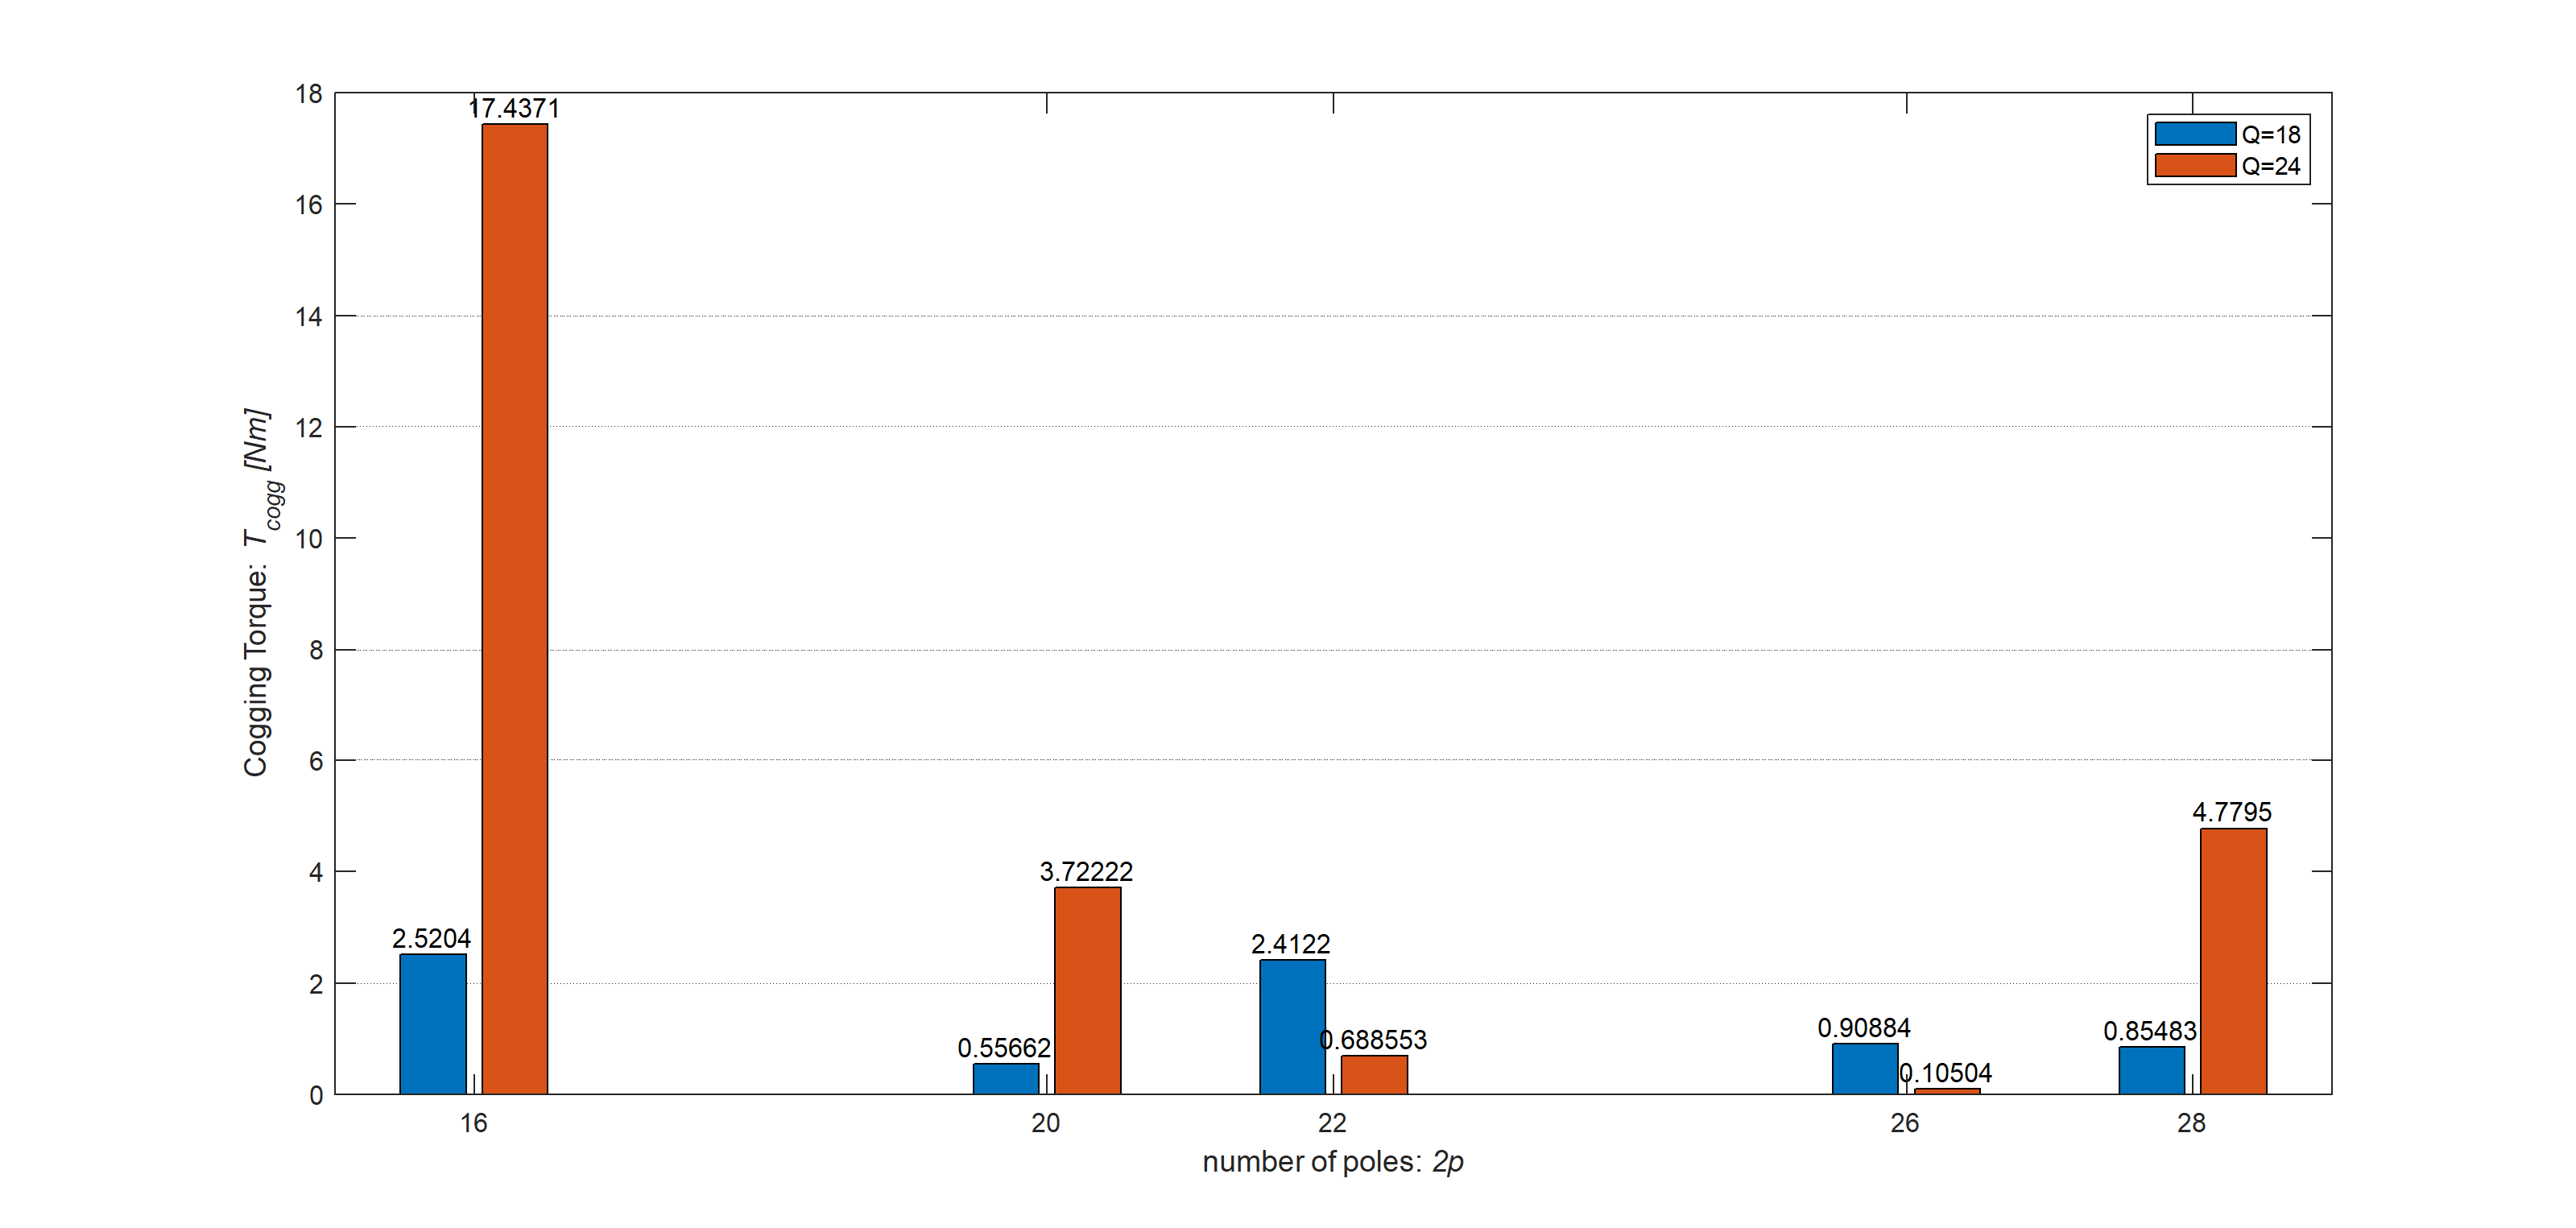
\includegraphics[width=\textwidth]{Tcogg_lvl1.png}
		\caption{Cogging Torque $T_{cogging}$ for different slot $Q$ and pole $2p$ values}
		\label{fig:coggingTorquelvl1}
	\end{figure}
	
	
	
	\section{Comparison \& Discussion}
	
	\subsection{Further Cogging Torque Optimization: Utilizing Skewed Stators}
	
	Jahns and Soong (1996) reports skewing method as one of the most effective one to reduce the cogging torque \cite{jahns_pulsating_1996}. Therefore; here, skewing method is utilized on the stator to further improve the EM in terms of cogging torque. To analyse skewing method on the selected EM in terms of cogging torque $T_{cogging}$, several skew widths are utilized. These skew widths are: half, one, two and three, period of cogging torque in the EM with no skew. These widths and the resulting cogging torque values can be seen in Tab. \ref{tab:resultslvl2}. The resulting cogging torque $T_{cogging}$ between two teeth can be seen in Fig. 
	
	\begin{table}[h]
		\begin{center}
			\begin{tabular}{c|c|c|c}
				$Q/2p=24/26$ & $a_{sk,0}=0$ & $a_{sk,1/2}=0.3442$ & $a_{sk,1}=0.6883$ \\
				\hline
				Cogging Torque $T_{cogging} [mNm]$ & 104.819 & 9.244326 & 1.97881 \\
				\hline\hline
				 & $a_{sk,2}=0.0014$ & $a_{sk,3}=0.0021$ \\
				\hline
				Cogging Torque $T_{cogging} [mNm]$ & 0 & 0\\
			\end{tabular}
		\end{center}
		\caption{Results: Cogging Torque $T_{cogging}$ for different skew widths $a_{sk}$}
		\label{tab:resultslvl2}
	\end{table}
	
	The results comply with what Azar, Zhu and Ombach (2012) reported \cite{azar_influence_2012}. Skewing stator side for a width corresponding to one actual period of cogging torque of the EM without skew significantly reduces the cogging torque $T_{cogging}$, if not, eliminate. As can be seen in Tab. \ref{tab:resultslvl2}, in the analysed EMs with skew width corresponds to 2 and 3 actual period of the cogging torque $T_{cogging}$ in the EM with no skew, the results show that cogging torque is completely eliminated.
	
	\begin{figure}
	     \centering
	     \begin{subfigure}[b]{1.0\textwidth}
	         \centering
	         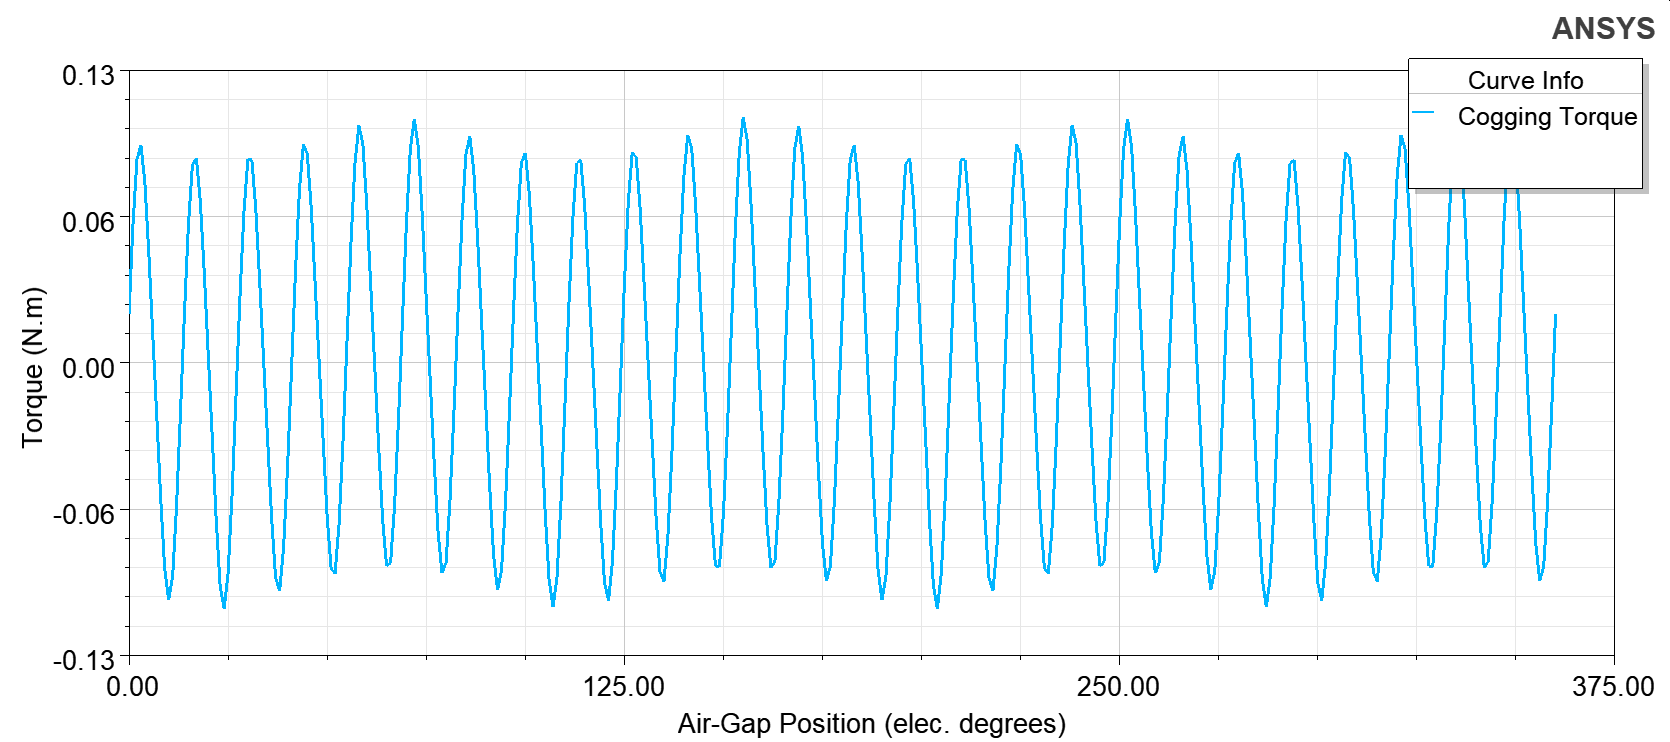
\includegraphics[height=3cm]{Tcogg_2426_a-0.png}
	         \caption{No Skew}
	         \label{fig:y equals x}
	     \end{subfigure}
	     \hfill
	     \begin{subfigure}[b]{1.0\textwidth}
	         \centering
	         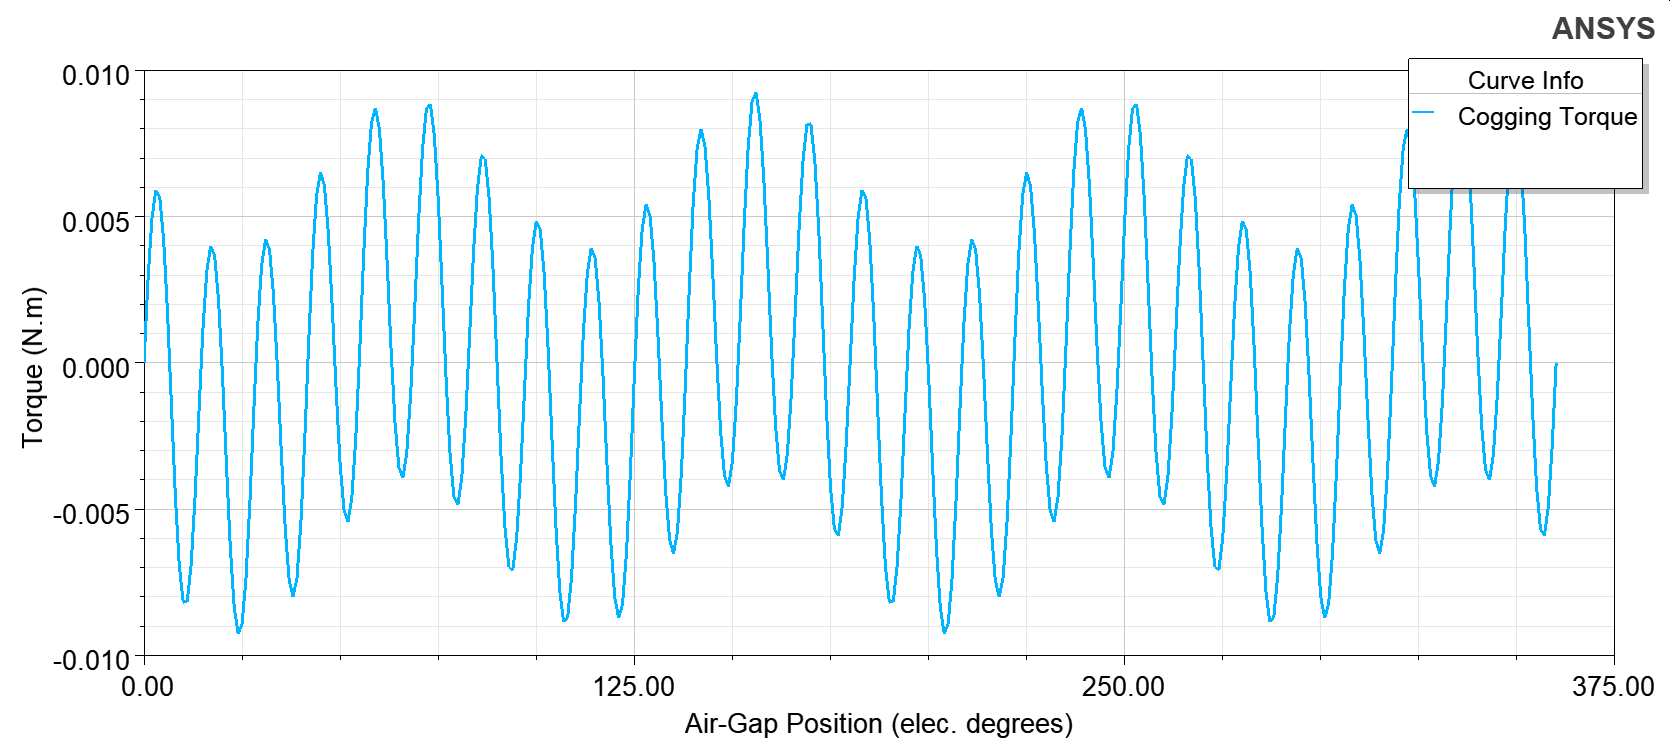
\includegraphics[height=3cm]{Tcogg_2426_a-half.png}
	         \caption{Skew: 1/2 period}
	         \label{fig:three sin x}
	     \end{subfigure}
	     \hfill
	     \begin{subfigure}[b]{1.0\textwidth}
	         \centering
	         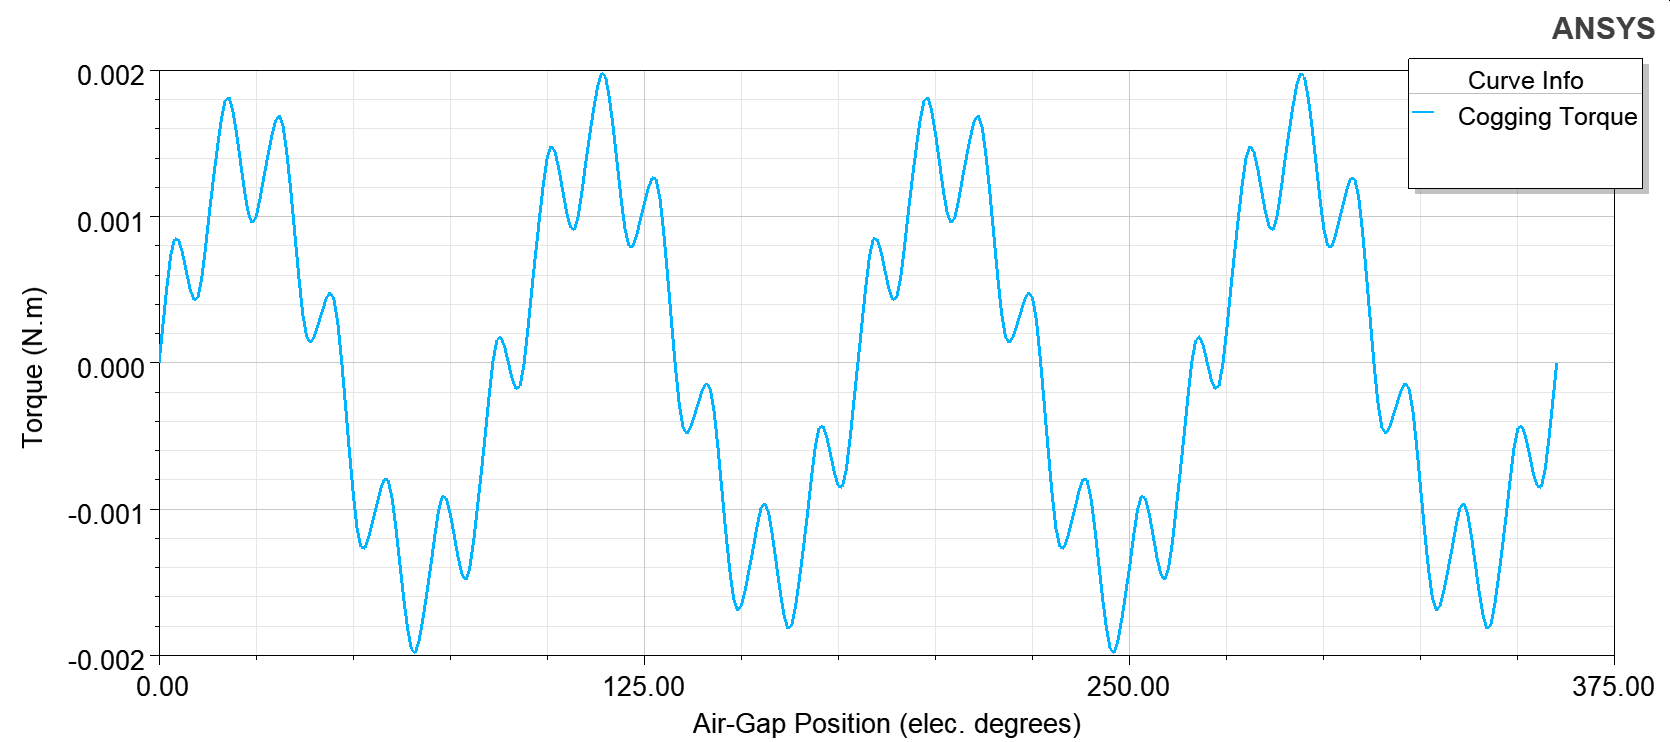
\includegraphics[height=3cm]{Tcogg_2426_a-1.png}
	         \caption{Skew: 1 period}
	         \label{fig:five over x}
	     \end{subfigure}
	     \hfill
	     \begin{subfigure}[b]{1.0\textwidth}
	         \centering
	         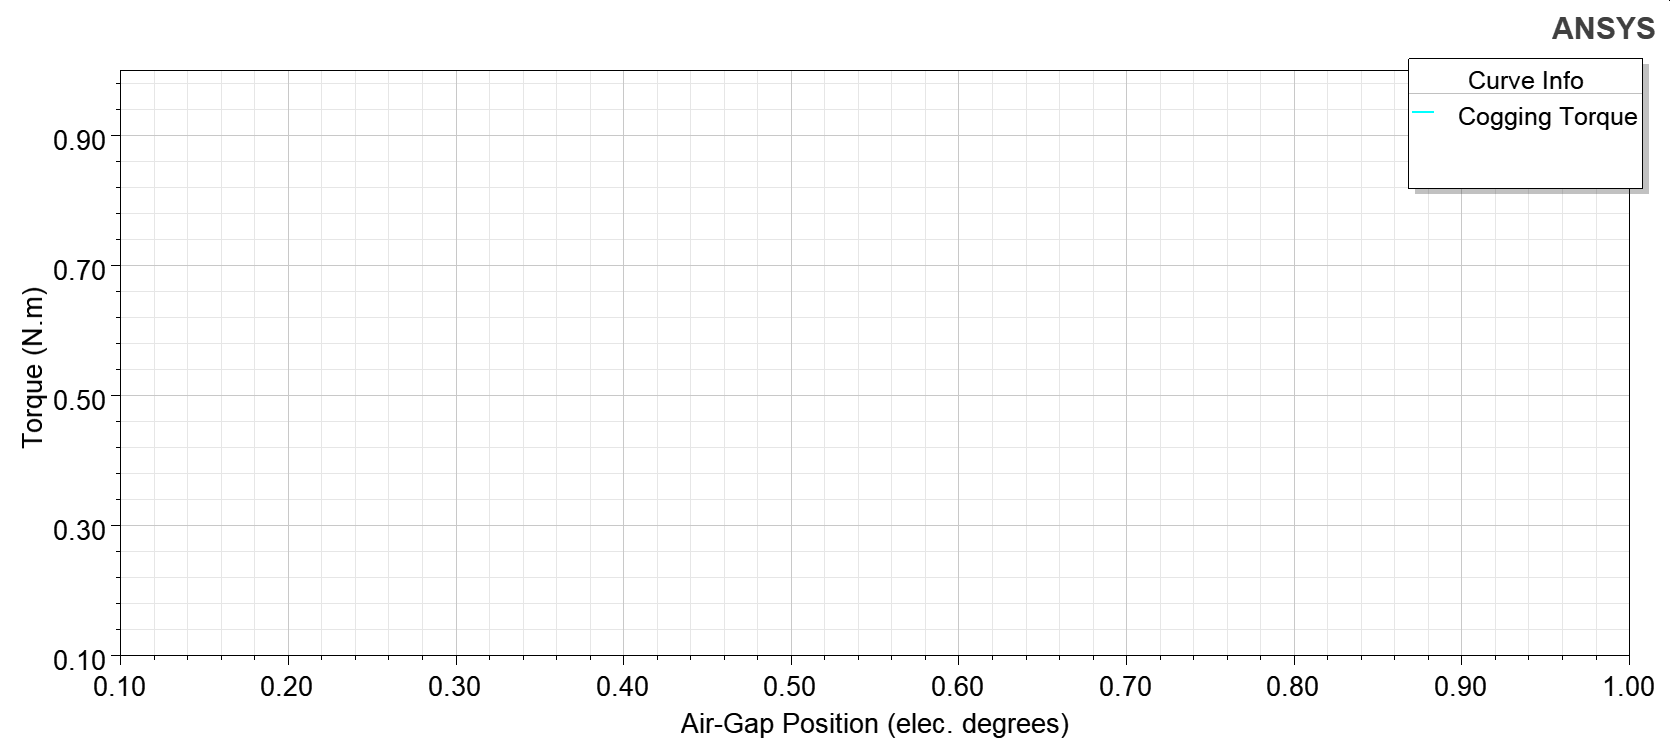
\includegraphics[height=3cm]{Tcogg_2426_a-2.png}
	         \caption{Skew: 2 period}
	         \label{fig:five over x}
	     \end{subfigure}
	     \hfill
	     \begin{subfigure}[b]{1.0\textwidth}
	         \centering
	         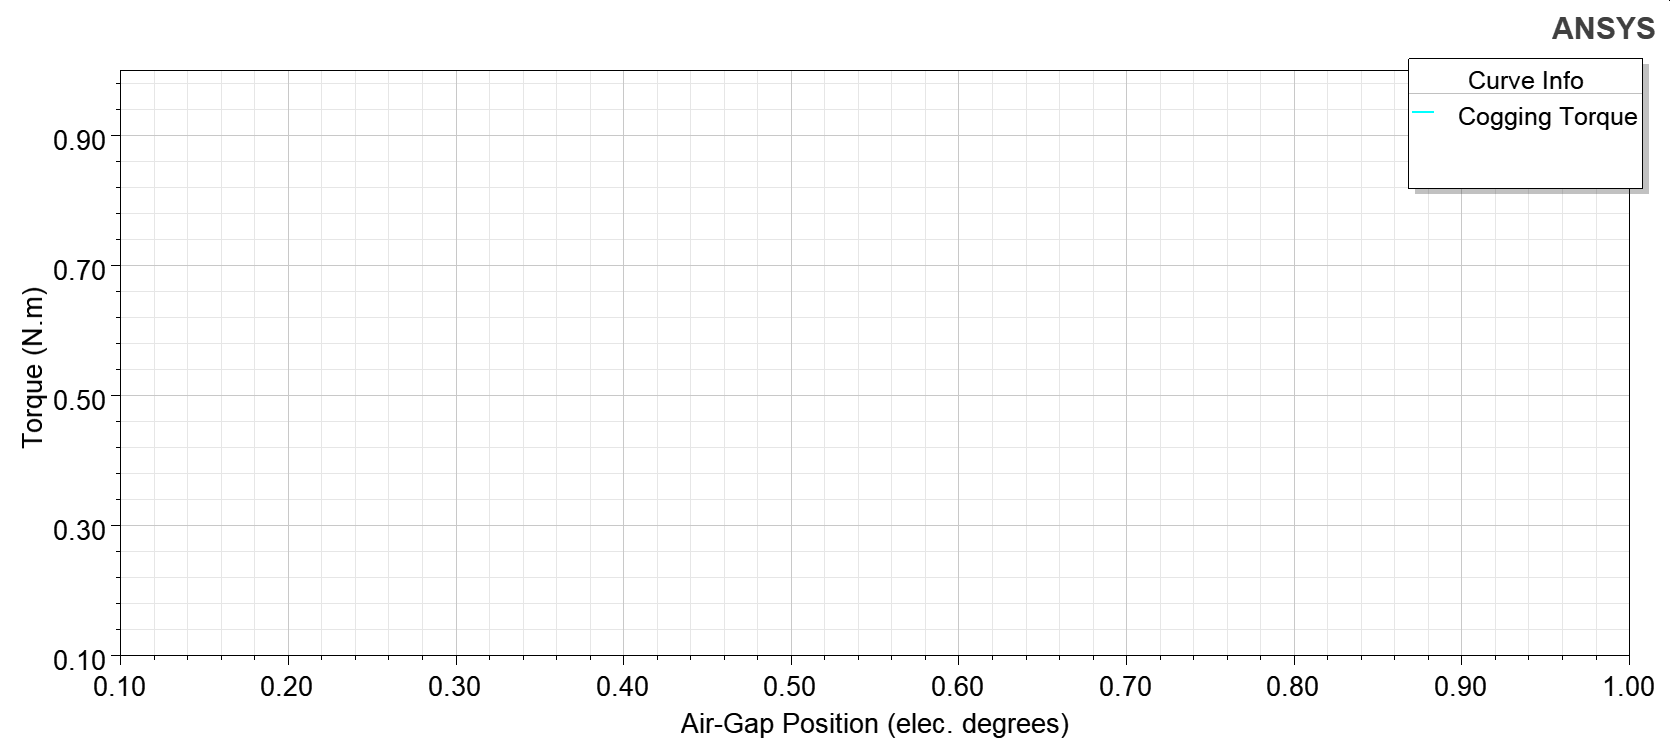
\includegraphics[height=3cm]{Tcogg_2426_a-3.png}
	         \caption{Skew: 3 period}
	         \label{fig:five over x}
	     \end{subfigure}
	        \caption{Skewing and corresponding Cogging Torque $T_{cogging}$}
	        \label{fig:coggingTorque}
	\end{figure}
	
	The corresponding skew factor $k_{skew}$ can be calculated as follows,
	\begin{equation}
		k_{skew}=\frac{sin(n\frac{\theta_{skew}}{2})}{n\frac{\theta_{skew}}{2}}
	\end{equation}
	where, $n$ is the harmonic order and $\theta_{skew}$ is the skew angle. The skew widths presented in \ref{tab:resultslvl2} are very small (one period of the actual cogging torque is $1/26$ of the tooth width, and the tooth width is $1/48$ of $2\pi$, resulting with $\pi/624$ rad.), such that the effect of mentioned skewing can be disregarded.
	
	
	\subsection{Further Dimensional Optimization: Increasing Stator Teeth and Yoke Flux Density} 
	
	Flux densities of the designed EM and the permitted flux densities at critical parts of the stator can be seen in Tab. \ref{tab:fluxDensityinCrit.1}. These values can both be increased further, while they are below the permitted flux densities \cite{pyrhonen_design_2014}. Therefore, the stator tooth width is scaled down by a factor of 80\% and and stator back-iron height is scaled down by a factor of 60\%. Old and new stator tooth widths and back-iron heights, and the corresponding flux densities can be seen in Tab.
	
	\begin{table}[h]
		\begin{center}
			\begin{tabular}{c|c|c}
				& Flux Density $B [T]$ & Permitted Flux Density $B [T]$ \\
				\hline
				Stator Teeth & 1.2893 & 1.6-2.0\\
				\hline\hline
				Stator Yoke & 0.5148 & 1.0-1.5\\
			\end{tabular}
		\end{center}
		\caption{Flux Density in Stator Teeth and Stator Yoke \cite{pyrhonen_design_2014}}
		\label{tab:fluxDensityinCrit.1}
	\end{table}
	
	\begin{table}[h]
		\begin{center}
			\begin{tabular}{c|c|c|c|c}
				& old dimension [mm] & new dimension [mm] & Old Flux Density $B [T]$ & New Flux Density $B [T]$ \\
				\hline
				Stator Teeth & 17.9 & 14.32 & 1.2893 & 1.6253 \\
				\hline\hline
				Stator Yoke & 17.9 & 10.74 & 1.1497 \\
			\end{tabular}
		\end{center}
		\caption{Flux Density in Stator Teeth and Stator Yoke \cite{pyrhonen_design_2014}}
		\label{tab:fluxDensityinCrit.1}
	\end{table}
	
	\subsection{Final Design}
	
	\paragraph{Mechanical Parameters} can be seen in Tab. \ref{tab:finalMechPara}
	
	\begin{table}[h]
		\begin{center}
			\begin{tabular}{c|c}
				Outer Diameter $[mm]$ & 403.01 \\
				Axial length $[mm]$ & 42.2 \\
				Aspect ratio & 0.154 \\
				Total Volume $[m^3]$ & 0.0054 \\
				\hline\hline
				Material mass & \\
				Armature Copper Weight $[kg]$ & 9.74326 \\
				Permanent Magnet Weight $[kg]$ & 2.36995 \\
				Armature Core Steel Weight $[kg]$ & 9.01669 \\
				Rotor Core Steel Weight $[kg]$ & 12.4689 \\
				Total New Weight $[kg]$ & 33.5991 \\
				\hline\hline
				Torque density $[Nm/m^3]$ & 30888 \\
				Power density $[kW/m^3]$ & 9516.3 \\
			\end{tabular}
		\end{center}
		\caption{Mechanical Parameters of the Final Design}
		\label{tab:finalMechPara}
	\end{table}
	
	
	\paragraph{Air-gap Flux Density Distribution} can be seen in Fig. \ref{fig:airgapFluxDensityDist}. The peak air-gap flux density is $\hat{B}_g\approx0.956T$. The magnet arcs are determined to be $0.6$, and as can be seen, it alters the air-gap flux density distribution from a trapezoidal to a more sinusoidal form.
	
	\begin{figure}[h]
		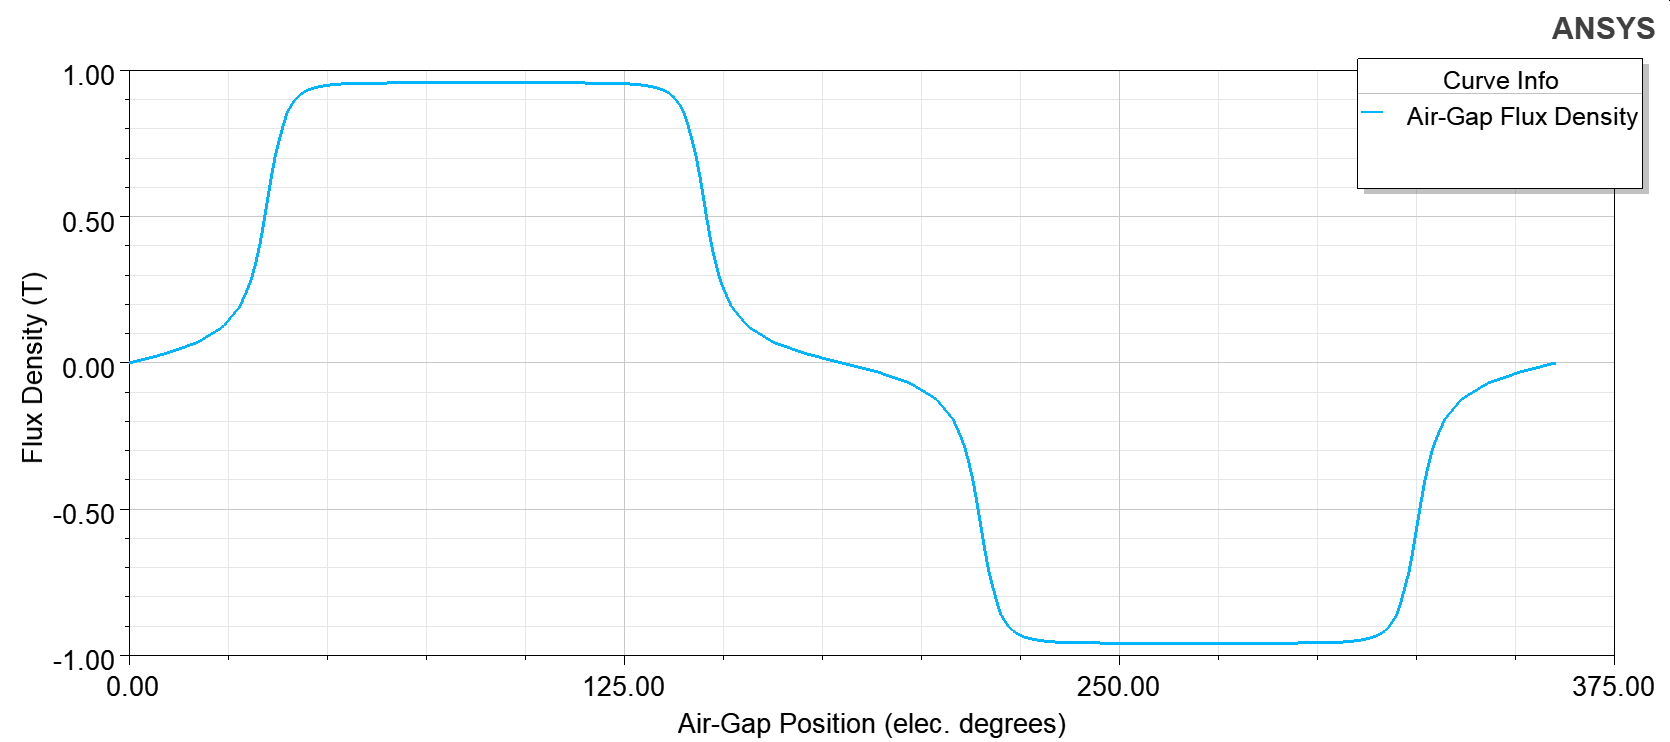
\includegraphics[width=\textwidth]{airgapFluxDensityDist.png}
		\caption{Air-gap Flux Density Distribution}
		\label{fig:airgapFluxDensityDist}
	\end{figure}
	
	\paragraph{Flux density distribution: Stator Teeth, Stator Yoke and Rotor Yoke} can be seen in Tab. \ref{tab:fluxDensityinCrit.}
	
	
	\begin{table}[h]
		\begin{center}
			\begin{tabular}{c|c}
				& Flux Density $B$ \\
				\hline
				Stator Teeth $[T]$ & 1.6253 \\
				\hline\hline
				Stator Yoke $[T]$ & 1.1497 \\
				\hline
				Rotor Yoke $[T]$ & 0.1170 \\
			\end{tabular}
		\end{center}
		\caption{Flux Density in Stator Teeth, Stator Yoke and Rotor Yoke}
		\label{tab:fluxDensityinCrit.}
	\end{table}
	
	
	\paragraph{Phase resistance and Inductances} can be seen in Tab. \ref{tab:phRandL}
	
	\begin{table}[h]
		\begin{center}
			\begin{tabular}{c|c}
				Phase resistance $[m\Omega]$ & 17.879 \\
				\hline\hline
				d-axis reactive inductance $L_{ad} [nH]$ & 73929.7 \\
				\hline
				q-axis reactive inductance $L_{aq} [nH]$ & 450106 \\
				\hline
				d-axis inductance $L_1+L_{ad} [nH]$ & 5079620 \\
				\hline
				q-axis inductance $L_1+L_{aq} [nH]$ & 5455800 \\
				\hline
				armature leakage inductance & 5005690 \\
			\end{tabular}
		\end{center}
		\caption{Phase Resistances and Inductances}
		\label{tab:phRandL}
	\end{table}
	
	\paragraph{Induced Phase and Line Voltages} can be seen in Fig. \ref{fig:inducedPhL2lV}
	\begin{figure}[h]
		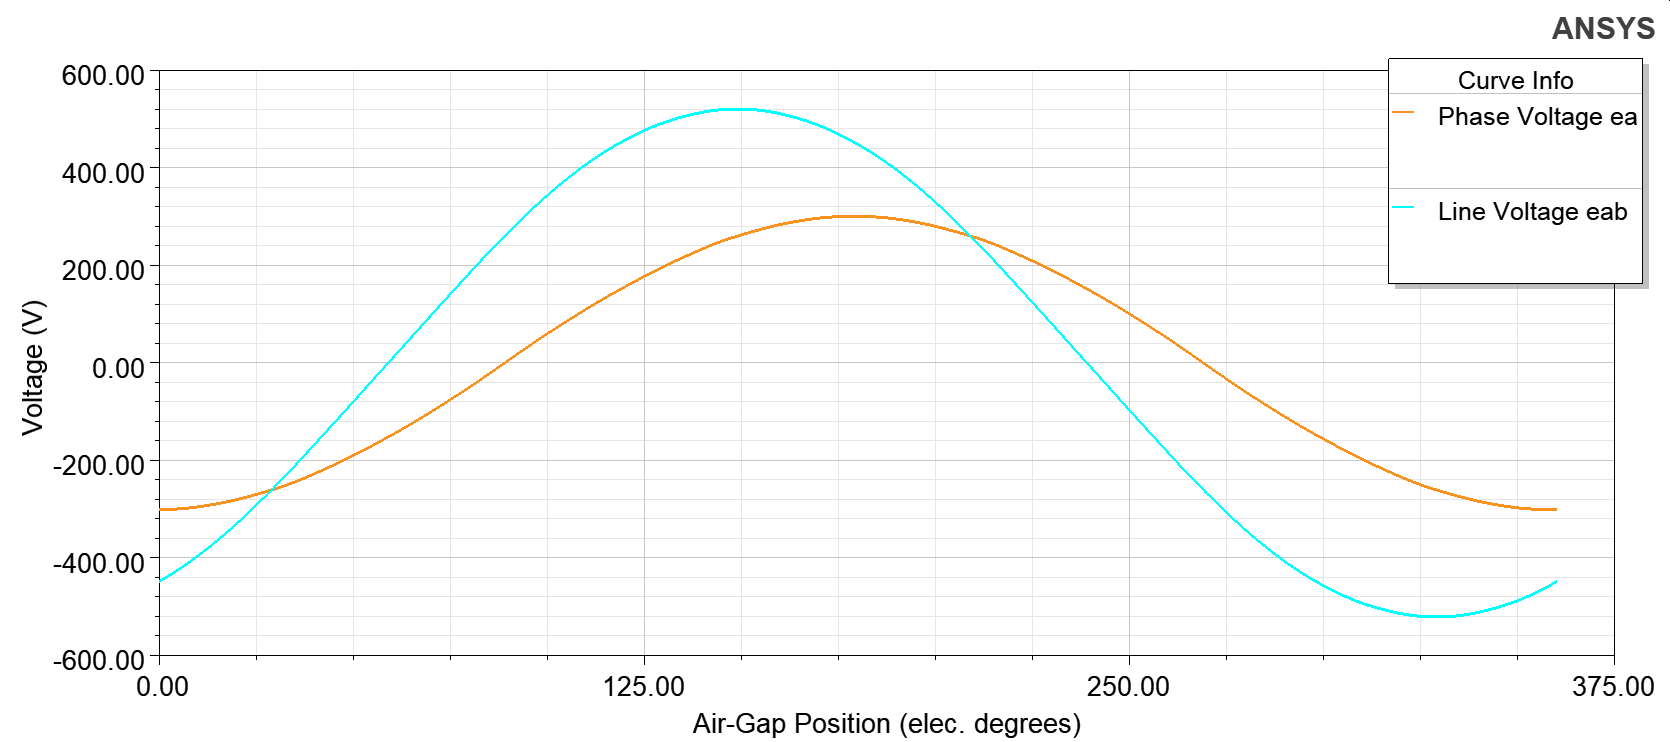
\includegraphics[width=\textwidth]{inducedVoltages.png}
		\caption{Induced Phase and Line Voltages}
		\label{fig:inducedPhL2lV}
	\end{figure}
	
	
	\paragraph{Efficiency calculation} can be seen in Tab. \ref{tab:effCalc}. 
	\begin{table}[h]
		\begin{center}
			\begin{tabular}{c|c}
				Iron-Core Loss $[W]$ & 314.106 \\
				\hline
				Armature Copper Loss $[W]$ & 259.591 \\
				\hline
				Total Loss $[W]$ & 573.697 \\
				\hline
				Output Power $[W]$ & 47013.5 \\
				\hline
				Input Power $[W]$ & 47587.2 \\
				\hline
				Efficiency $[\%]$ & 98.7944 \\
			\end{tabular}
		\end{center}
		\caption{Losses and Efficiency at Full-Load}
		\label{tab:effCalc}
	\end{table}
	
	\paragraph{Maximum Power} this machine can provide is $P_{max}=51227.5W$. The output power with respect to torque angle can be seen in Fig. \ref{fig:PvsTangle}.
	\begin{figure}[h]
		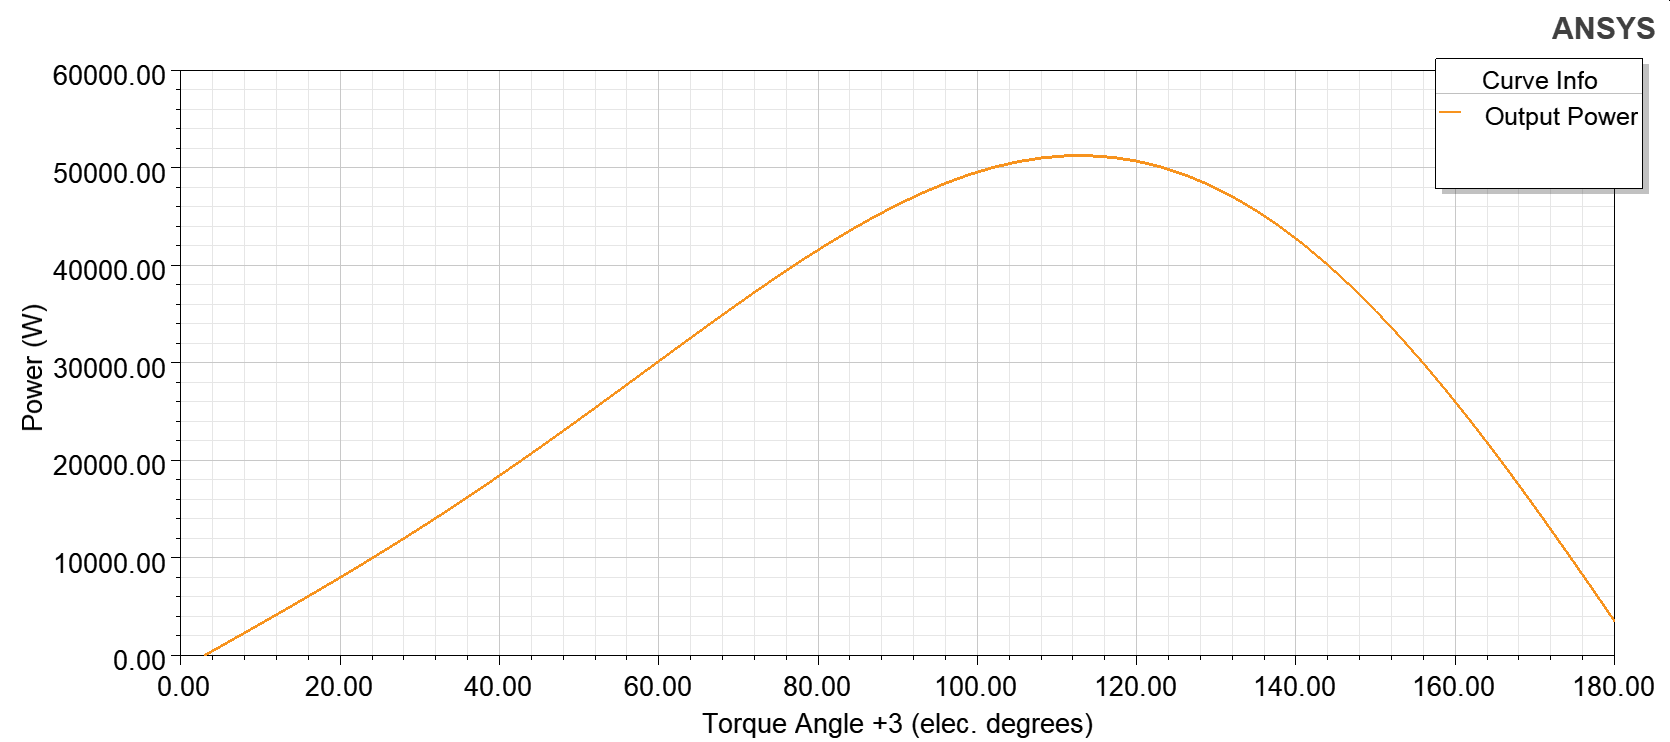
\includegraphics[width=\textwidth]{maxpower.png}
		\caption{Power vs. Torque Angle}
		\label{fig:PvsTangle}
	\end{figure}
	
	\subsection{Evaluation of the Design}
	
	The bridge and the rib dimensions are chosen throughout the research without a mechanical analysis. To achieve the required air-gap flux density, these dimensions are significantly lowered, and it is highly probable that the current dimensions may not able to hold the PMs and the rotor intact. A mechanical stress analysis is required to be performed on the rotor bridge and rib to analyse the maximum speed they can endure, and their dimensions are to be increased, if needed. In the case that the bridge and rib dimensions are increased, the resulting air-gap flux density $B_g$ is lower than its current value due to the increased pole leakage flux. Thefore, new methods shall be required to achieve the current air-gap flux density $B_g$ values. Most straightforward method is to use v-shaped IPM rotor instead of flat-shaped.
		
	\section{Conclusion}
	
	In this paper, an EM for a hybrid electric propulsion system is designed. Different stator slot/pole configurations are analysed with single-layer FSCW topology and compared in terms of cogging torque. It is verified that the cogging torque can be assessed with the cogging torque factor introduced by Zhu and Howe (2000) \cite{zhu_influence_2000}. Furthermore, cogging torque is completely eliminated via. skewing the stator for a width of actual cogging torque period, verifying the work of Azar, Zhu and Ombach (2012) \cite{azar_influence_2012}. Final design is further optimized as the flux density in stator teeth and yoke are below the permitted level. To achieve higher flux densities at these areas, stator teeth width and back-iron height is scaled down. Overall, a single-layer FSCW-IPMSM is designed with an efficiency of $\approx98.8\%$.



	\newpage
	
	\bibliography{bibliography} 
	\bibliographystyle{ieeetr}
\end{document}